%% ============================================================
% f2012_shandong_arts_q21_ellipse.tex
%% 2012 山东卷（文科）第 21 题 椭圆 M 与矩形 ABCD
%% 来源 PDF：普通高考/2012/2012山东文.pdf 第 2 页（印面 762）第 2 栏
%% 坐标取自原页矢量层（bp），原点为图区左上角 (615.0,485.0)，y 向下。
%% ============================================================
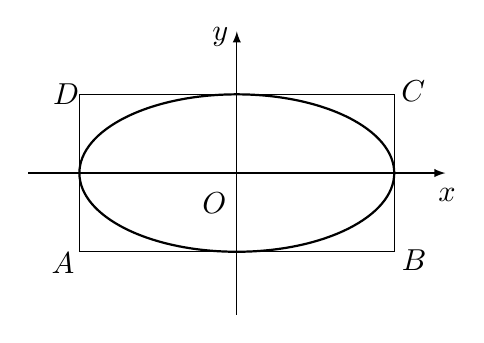
\begin{tikzpicture}[x=1bp,y=-1bp,
  every node/.style={inner sep=0,font=\fontsize{10.5pt}{12.6pt}\selectfont},
  line cap=butt, line join=miter]
  \draw[line width=0.3985bp] (4.234,65.039) -- (150.832,65.039);
  \fill[black] (154.418,65.039) .. controls (153.355,64.84) and (151.629,64.242) .. (150.434,63.547) -- (150.434,66.535) .. controls (151.629,65.836) and (153.355,65.238) .. (154.418,65.039);
  \draw[line width=0.3985bp] (79.328,116.047) -- (79.328,17.621);
  \fill[black] (79.328,14.035) .. controls (79.129,15.098) and (78.531,16.824) .. (77.832,18.02) -- (80.82,18.02) .. controls (80.125,16.824) and (79.527,15.098) .. (79.328,14.035);
  \draw[line width=0.797bp] (136,65.039) .. controls (136,49.391) and (110.625,36.703) .. (79.328,36.703) .. controls (48.027,36.703) and (22.656,49.391) .. (22.656,65.039) .. controls (22.656,80.691) and (48.027,93.375) .. (79.328,93.375) .. controls (110.625,93.375) and (136,80.691) .. (136,65.039) -- cycle;
  \draw[line width=0.3985bp] (22.656,93.375) -- (22.656,36.703) -- (136,36.703) -- (136,93.375) -- cycle;
  \node[anchor=base west] at (70.37,17.4) {$y$};
  \node[anchor=base west] at (138.36,39.15) {$C$};
  \node[anchor=base west] at (13.02,40.3) {$D$};
  \node[anchor=base west] at (151.71,75.4) {$x$};
  \node[anchor=base west] at (66.74,79.49) {$O$};
  \node[anchor=base west] at (138.53,100.05) {$B$};
  \node[anchor=base west] at (12.42,101.2) {$A$};
\end{tikzpicture}
